\documentclass{article}%
\usepackage[T1]{fontenc}%
\usepackage[utf8]{inputenc}%
\usepackage{lmodern}%
\usepackage{textcomp}%
\usepackage{lastpage}%
\usepackage[head=40pt,margin=0.5in,bottom=0.6in]{geometry}%
\usepackage{graphicx}%
%
\title{\textbf{Trabajadores protestan para exigir la libertad de Rubén González}}%
\author{El Nacional Web}%
\date{03/12/2018}%
%
\begin{document}%
\normalsize%
\maketitle%
\textbf{URL: }%
http://www.el{-}nacional.com/noticias/protestas/trabajadores{-}protestan{-}para{-}exigir{-}libertad{-}ruben{-}gonzalez\_261931\newline%
%
\textbf{Periodico: }%
EN, %
ID: %
261931, %
Seccion: %
Protestas\newline%
%
\textbf{Palabras Claves: }%
Presos políticos, Gobierno\newline%
%
\textbf{Derecho: }%
1.2, %
Otros Derechos: %
2.3, %
Sub Derechos: %
1.2.2, 2.3.3\newline%
%
\textbf{EP: }%
SI\newline%
\newline%
%
\textbf{\textit{Los empleados piden al defensor del pueblo, Alfredo José Angulo, una respuesta sobre el sindicalista}}%
\newline%
\newline%
%
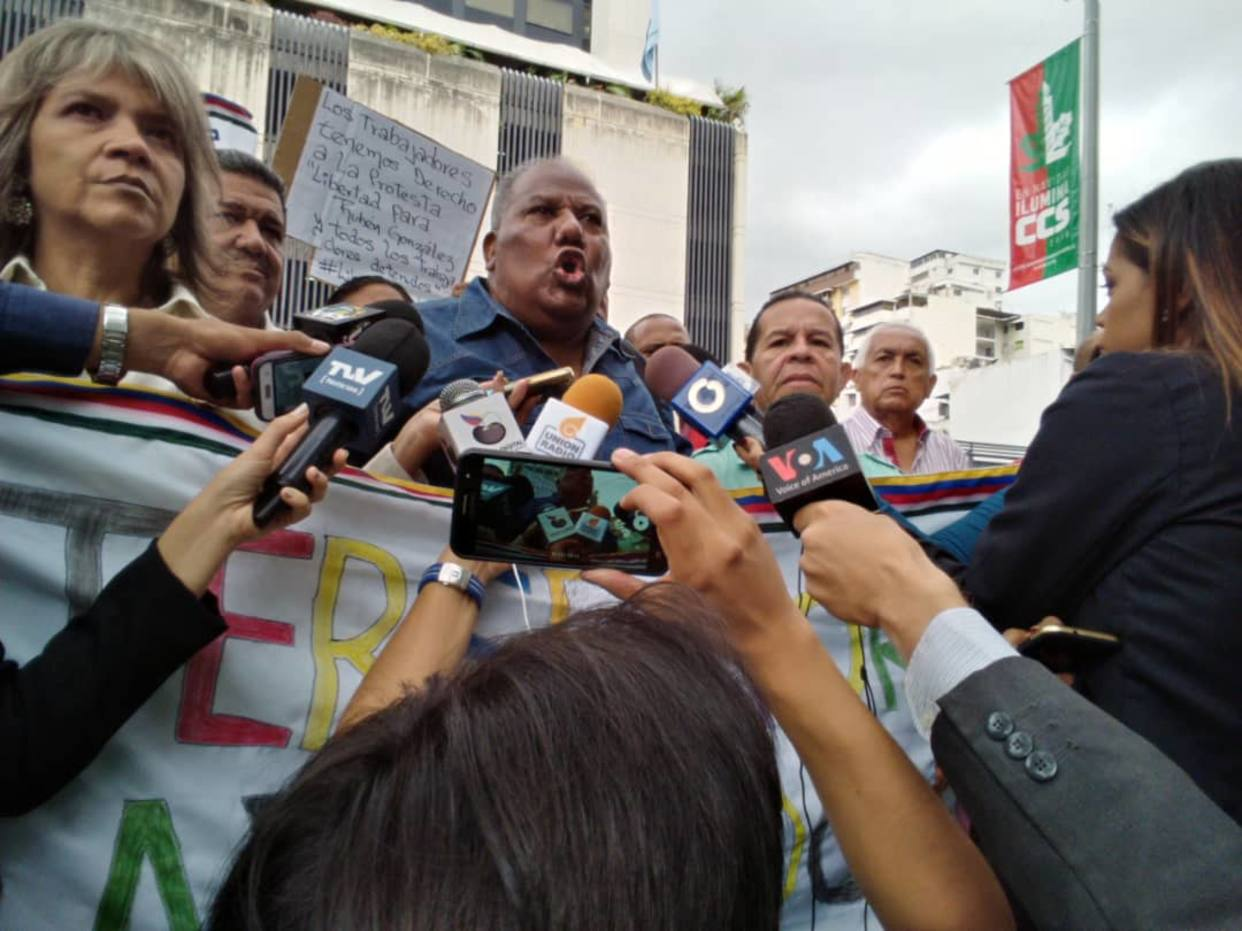
\includegraphics[width=300px]{207.jpg}%
\newline%
%
Trabajadores de la intersectorial de Venezuela protestan este lunes para exigir la liberación del sindicalista de Ferrominera, Rubén González.%
\newline%
%
"Rubén González solamente expresó en una rueda de prensa las desgracias que vive el sector trabajador", reveló un trabajador.%
\newline%
%
Los manifestantes piden al defensor del pueblo, Alfredo José Ruíz Angulo, respuesta sobre el estado de González.%
\newline%
%
Juan Véliz, presidente del Sindicato de la Cantv, informó que~realizarán movilizaciones para defender los derechos de los trabajadores.%
\newline%
%
\end{document}